\chapter{System Design}
This chapter discusses the system design, analysing the various aspects of the project and purpose of each component such as the visualisation, the sorting algorithms, user authentication, the server, etc.

\section{Overview}
\begin{center}
    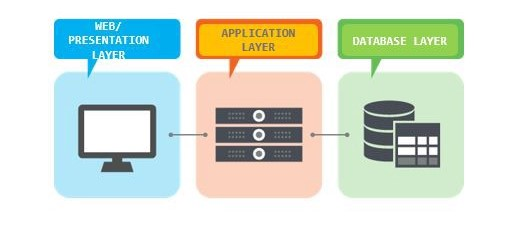
\includegraphics[width=8cm,height=3.3cm,keepaspectratio]{images/3tier}
\end{center}

This project utilises the multi-tier architecture (often referred to as n-tier architecture) platform. Multi-tier architecture or multilayered architecture is a client–server architecture in which presentation, application processing, and data management functions are physically separated. The most widespread use of multi-tier architecture is the three-tier architecture. This project consists of three main components, all working together: The web application, which represents the presentation layer, allows users to visualise various sorting algorithms, register and login, upload and view past sorts from other users. The Flask server, which represents the logic tier, handles requests such as account registration and log in, and uploading and retrieving of sorts by users. The databases: the MongoDB database which stores user details and the Firebase database which stores all previous sorts.

\begin{center}
    \includegraphics[width=15cm,height=17cm,keepaspectratio]{images/AppDesign}
\end{center}
\newpage

\section{Web Application}
The web application was designed and developed first as this is the main aspect of the project itself. The main objective of the web application was to allow a user to choose a sorting algorithm and be able to visualise it. Secondary objectives, which were developed at a later point, was to allow users to register and log in to an account, and have the ability to upload and view previous sorts. This was greatly aided by the decision to use ReactJS as discussed in Chapter 3 The web application consists of four main pages: 

\begin{itemize}
    \item \textbf{Sorting Page} - The sorting page, as shown in Figure \ref{fig:main_page}, is the main page of the application. Allows a user to choose one of several sorting algorithms to visualise, generate a random array of elements to sort, utilize the ScreenFlow API and specify their own dataset to sort.
    \item \textbf{Login Page} - The login page handles user authentication and will login a user to the application if that user exists within the database. The user will then be redirected to the sorting page, with new functionality available such as accessing the ScreenFlow API and uploading one's own dataset.
    \item \textbf{Register Page} - The register page handles user authentication and will register a user with the application. The user will then be redirected to the login page, where they can then attempt to login.
    \item \textbf{Sorts Page} - The sorts page displays all previous sorts recorded and saved by past users.
\end{itemize}

\begin{figure}[!h]
    \centering
    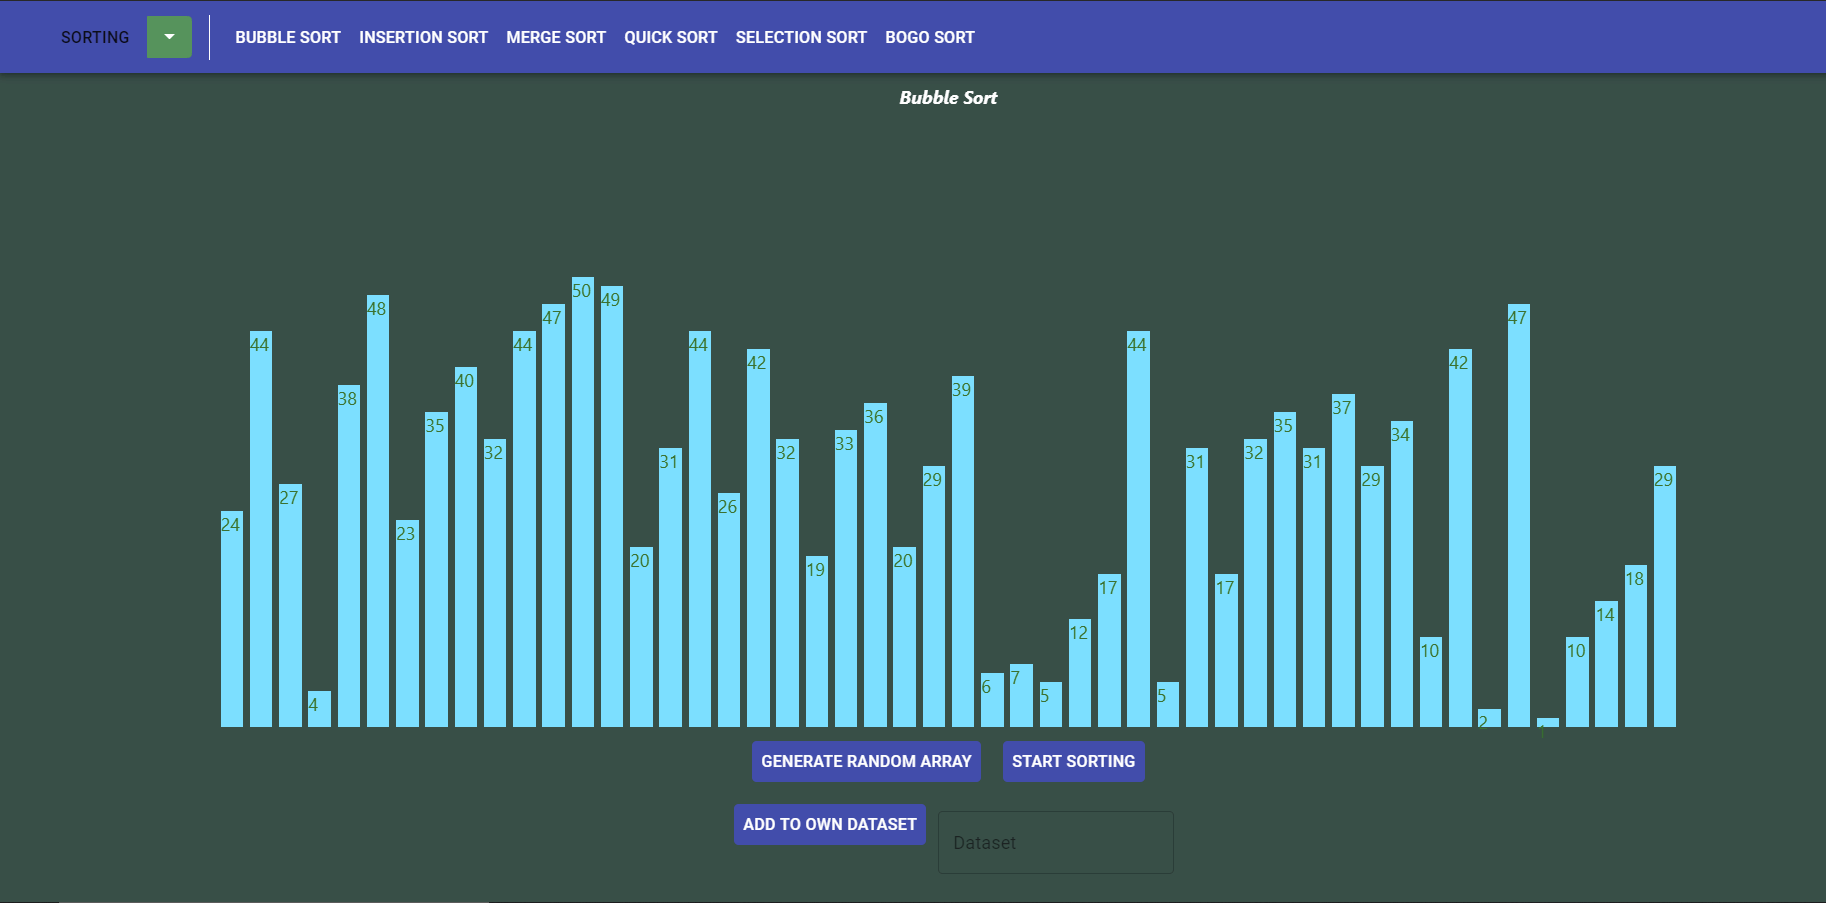
\includegraphics[scale=.35]{images/web_app_main}
    \label{fig:main_page}
\end{figure}

\subsection{Sorting}
\begin{center}
    \includegraphics[height=6.5cm,width=13cm]{images/sorting}
    \label{fig:main_page}
\end{center}
There are currently seven algorithms that can be visualised within the application. Currently, all sorting algorithms have been written using JavaScript \cite{sortalgs_guide}. They are as follows:

\begin{itemize}
    \item Bubble Sort \cite{bub_sor}
    \item Heap Sort
    \item Insertion Sort
    \item Merge Sort
    \item Quick Sort
    \item Selection Sort
    \item Shell Sort
\end{itemize}

\subsubsection{Bubble Sort}
\begin{center}
    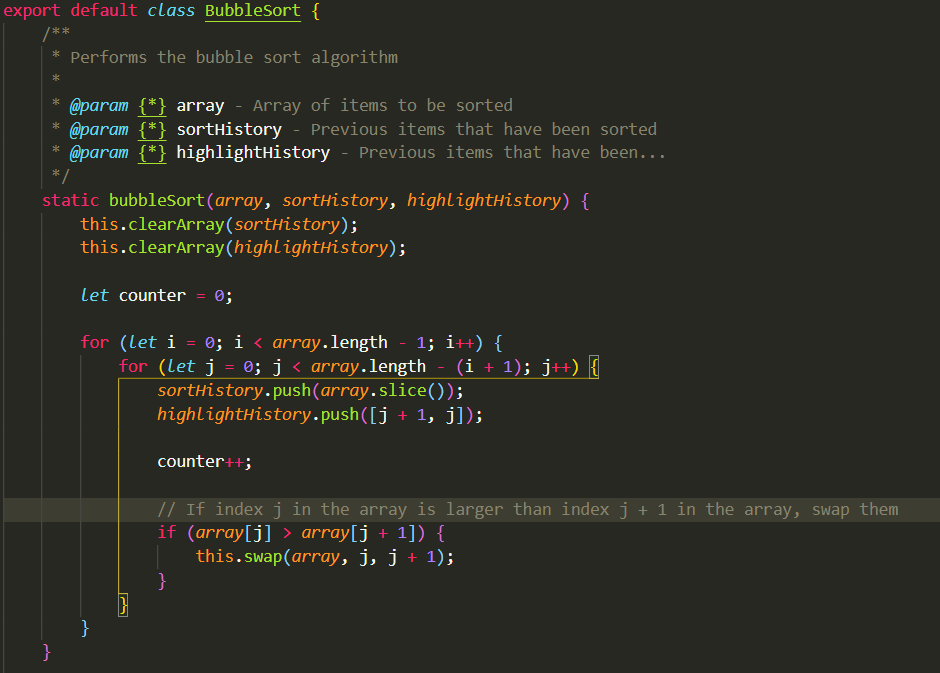
\includegraphics[width=12cm,height=15cm,keepaspectratio]{images/bubblesort}
\end{center}
Bubble sort, sometimes referred to as sinking sort, is a simple sorting algorithm that repeatedly steps through the list, compares adjacent elements and swaps them if they are in the wrong order \cite{bubble_sort}. The pass through the list is repeated until the list is sorted. The algorithm, which is a comparison sort, is named for the way smaller or larger elements "bubble" to the top of the list.
\par
\bigskip
This simple algorithm performs poorly in real world use and is used primarily as an educational tool. More efficient algorithms such as Tim Sort, or Merge Sort are used by the sorting libraries built into popular programming languages such as Python and Java.

\paragraph{How it works in the context of the application}
Bubble sort works by comparing adjacent pairs of objects in the array using nested for loops \cite{bubble_sort_geeks}. Sorted elements are pushed into \lstinline{sortedElements} as a new array object. Elements that need to be sorted are pushed into \lstinline{selectedElements}. If the objects are not in the correct ordered, they are swapped so that the largest of the two moves up.

% \subsubsection{Heap Sort}
% \begin{center}
%     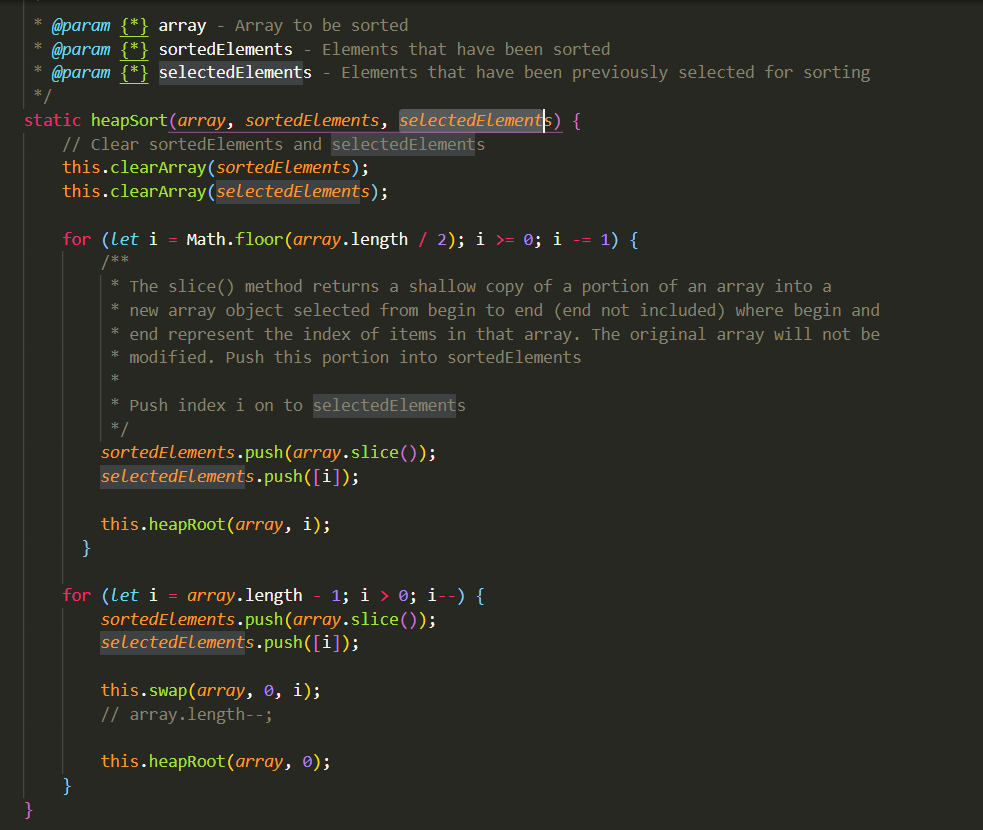
\includegraphics[width=6cm,height=8cm,keepaspectratio]{images/heapsort1}
%     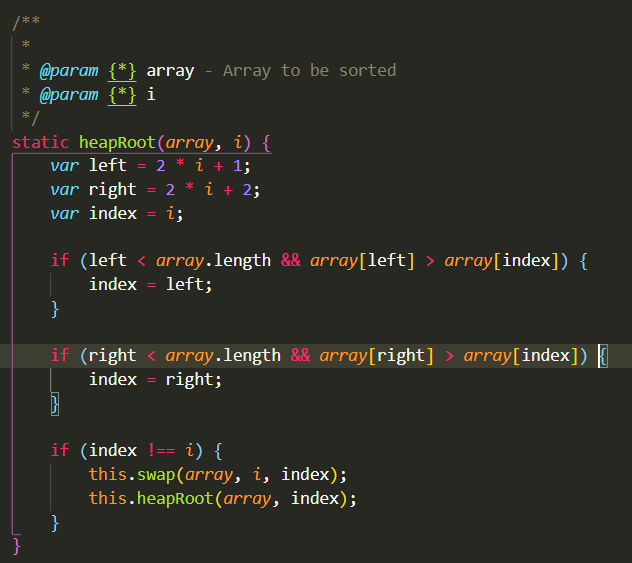
\includegraphics[width=6cm,height=8cm,keepaspectratio]{images/heapsort2}
% \end{center}
% Heap Sort is a comparison-based sorting algorithm. Heap Sort can be thought of as an improved Selection Sort: like Selection Sort, Heap Sort divides its input into a sorted and an unsorted region, and it iteratively shrinks the unsorted region by extracting the largest element from it and inserting it into the sorted region. Unlike Selection Sort, Heap Sort does not waste time with a linear-time scan of the unsorted region; rather, heap sort maintains the unsorted region in a heap data structure to more quickly find the largest element in each step.
% \par
% \bigskip
% Although somewhat slower in practice on most machines than a well-implemented Quick Sort, it has the advantage of a more favorable worst-case O(n log n) runtime. Heap Sort is an in-place algorithm, but it is not a stable sort.

% \paragraph{How it works in the context of the application}

\subsubsection{Insertion Sort}
\begin{center}
    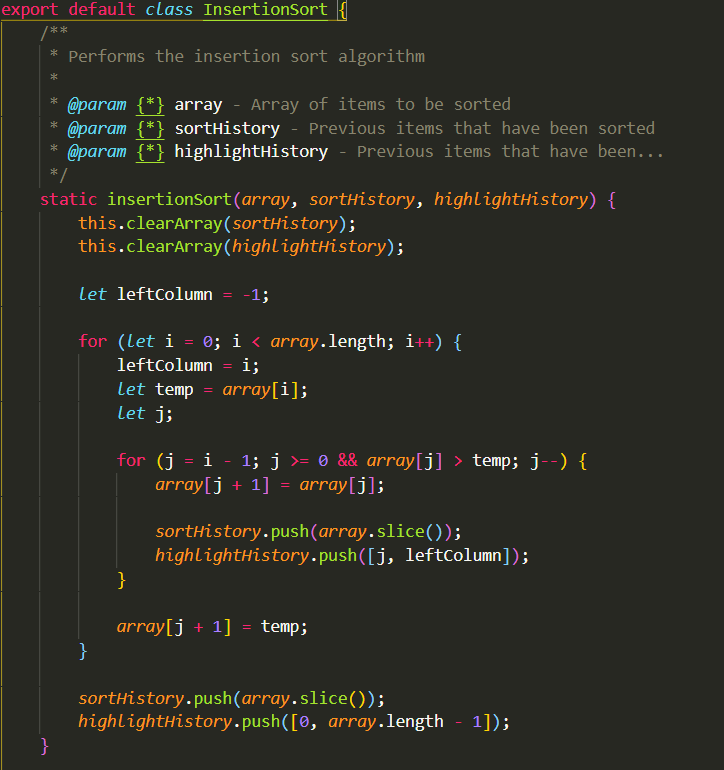
\includegraphics[width=12cm,height=15cm,keepaspectratio]{images/insertionsort}
\end{center}
Insertion sort is a simple sorting algorithm that builds the final sorted array (or list) one item at a time \cite{insertion_sort}. It is much less efficient on large lists than more advanced algorithms such as Quick Sort, Heap Sort, or Merge Sort. However, insertion sort provides several advantages:

\begin{itemize}
    \item \textbf{Efficient} - Efficient for (quite) small data sets, much like other quadratic sorting algorithms
    \item \textbf{Stable} - Does not change the relative order of elements with equal keys
    \item \textbf{Online} - Can sort a list as it receives it
    \item \textbf{Adaptive} - Efficient for data sets that are already substantially sorted:
\end{itemize}

When people manually sort cards in a bridge hand, most use a method that is similar to insertion sort.

\paragraph{How it works in the context of the application}
Insertion sort iterates, consuming one input element each repetition, and growing a sorted output list \cite{insertion_sort_geeks}. At each iteration, insertion sort removes one element from the input data, finds the location it belongs within the sorted list, and inserts it there. It repeats until no input elements remain.

\subsubsection{Merge Sort}
\begin{center}
    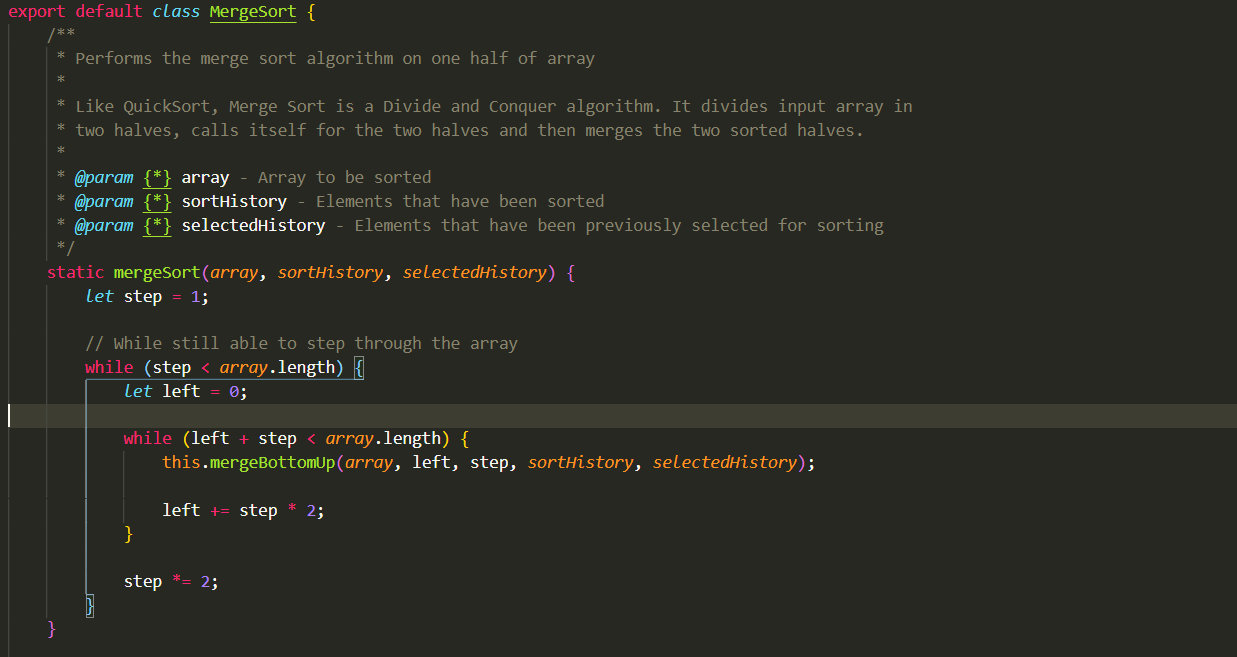
\includegraphics[width=12cm,height=6cm,keepaspectratio]{images/mergesort1}
    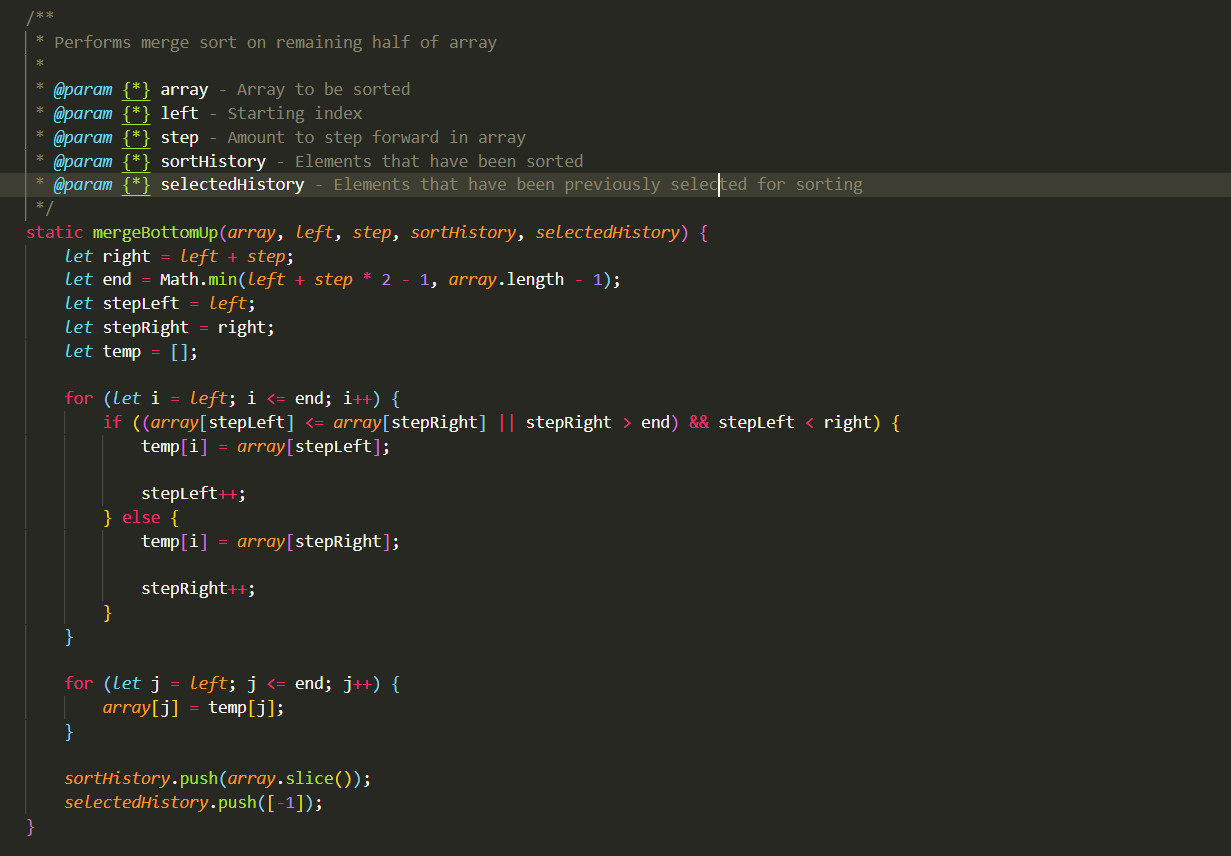
\includegraphics[width=12cm,height=6cm,keepaspectratio]{images/mergesort2}
\end{center}
Merge Sort is an efficient, general-purpose, comparison-based sorting algorithm \cite{merge_sort}. Most implementations produce a stable sort, which means that the order of equal elements is the same in the input and output. It divides input array in two halves, calls itself for the two halves and then merges the two sorted halves.

\paragraph{How it works in the context of the application}
A middle point is found and the array is divided in two halves. The sub-arrays are then recursively sorted in each of the two sub-problems created by the divide step. That is, recursively sort the sub-array \lstinline{array[p..q]} and recursively sort the sub-array \lstinline{array[q+1..r]}. The two sorted sub-arrays are then merged back into a single sorted array \cite{merge_sort_geeks}.

\subsubsection{Quick Sort}
\begin{center}
    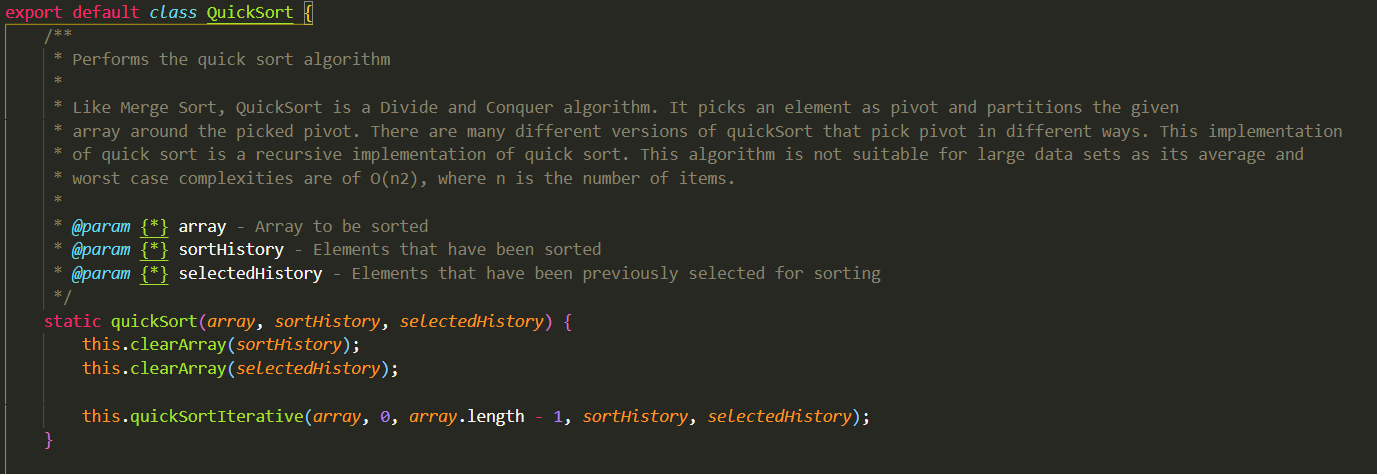
\includegraphics[width=12cm,height=12cm,keepaspectratio]{images/quicksort1}
    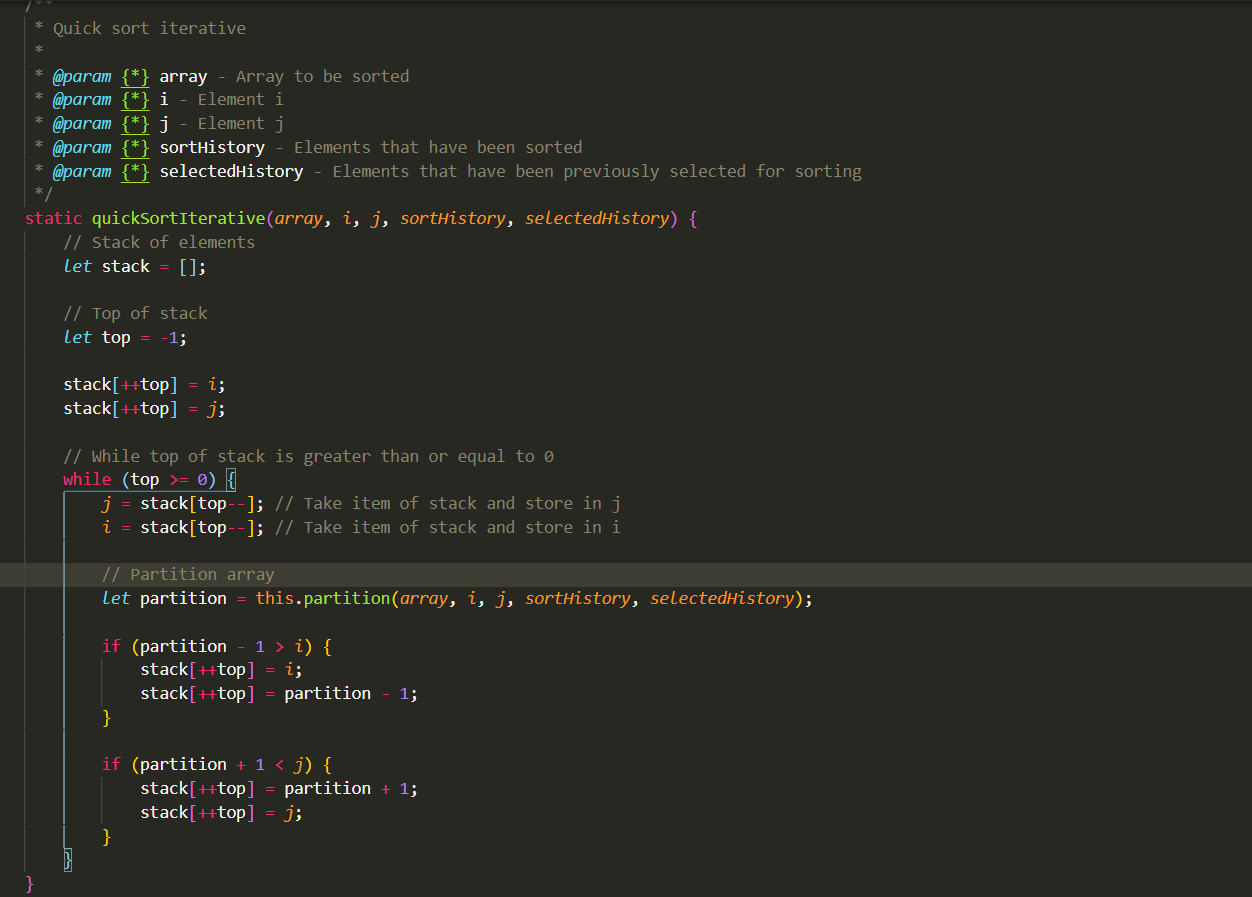
\includegraphics[width=12cm,height=12cm,keepaspectratio]{images/quicksort3}
    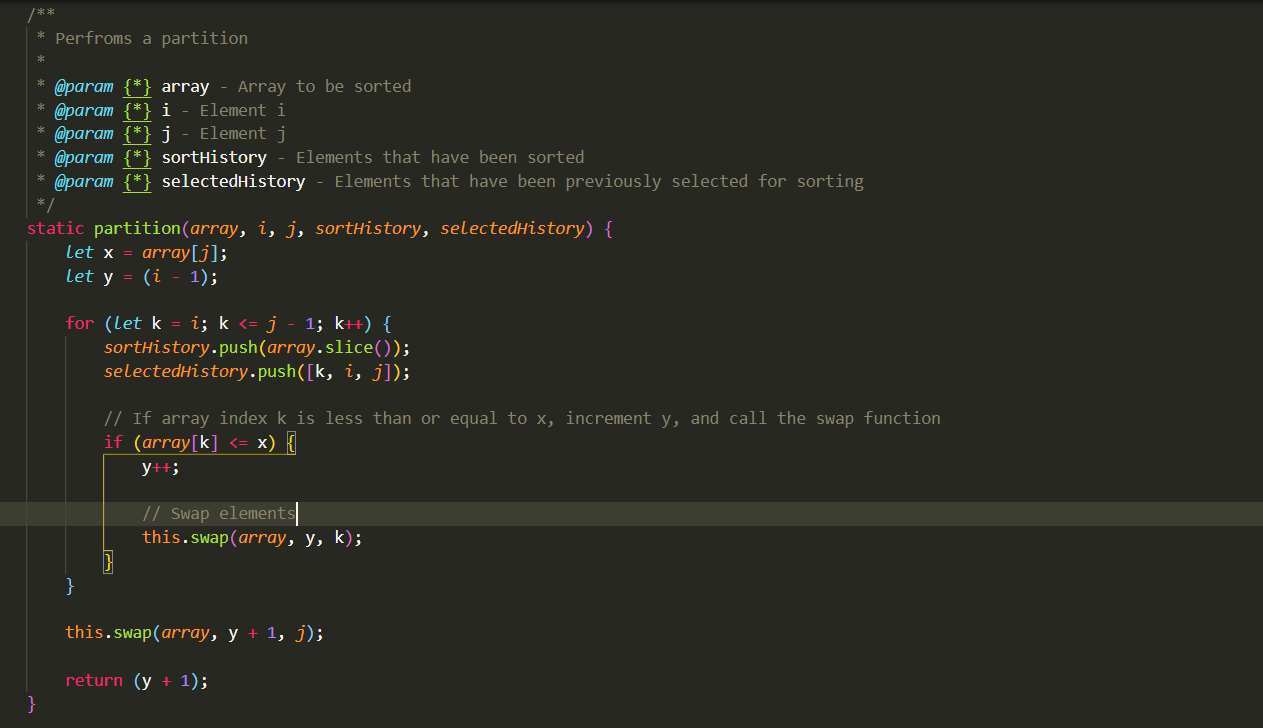
\includegraphics[width=12cm,height=12cm,keepaspectratio]{images/quicksort2}
\end{center}
Quick Sort is an efficient sorting algorithm \cite{quick_sort}.
Quick Sort is a divide-and-conquer algorithm. It works by selecting a 'pivot' element from the array and partitioning the other elements into two sub-arrays, according to whether they are less than or greater than the pivot. The sub-arrays are then sorted recursively. This can be done in-place, requiring small additional amounts of memory to perform the sorting.
\par
\bigskip
Quick Sort is a comparison sort, meaning that it can sort items of any type for which a "less-than" relation (formally, a total order) is defined. Efficient implementations of Quick Sort are not a stable sort, meaning that the relative order of equal sort items is not preserved.
\par
\bigskip
Mathematical analysis of Quick Sort shows that, on average, the algorithm takes O(n log n) comparisons to sort n items. In the worst case, it makes O(n2) comparisons, though this behavior is rare.

\paragraph{How it works in the context of the application}
A “pivot” item is found in the array. A left and right pointer is started in the first and last item in the array, respectively. While the value at the left pointer in the array is less than the pivot value, move the left pointer to the right (add 1). This continues until the value at the left pointer is greater than or equal to the pivot value. While the value at the right pointer in the array is greater than the pivot value, move the right pointer to the left (subtract 1). This continues until the value at the right pointer is less than or equal to the pivot value. If the left pointer is less than or equal to the right pointer, the values at these locations in the array are swapped. The left pointer  is moved to the right by one and the right pointer is moved to the left by one. If the left pointer and right pointer don’t meet, the process is started again \cite{quick_sort_geeks}.

\subsubsection{Selection Sort}
\begin{center}
    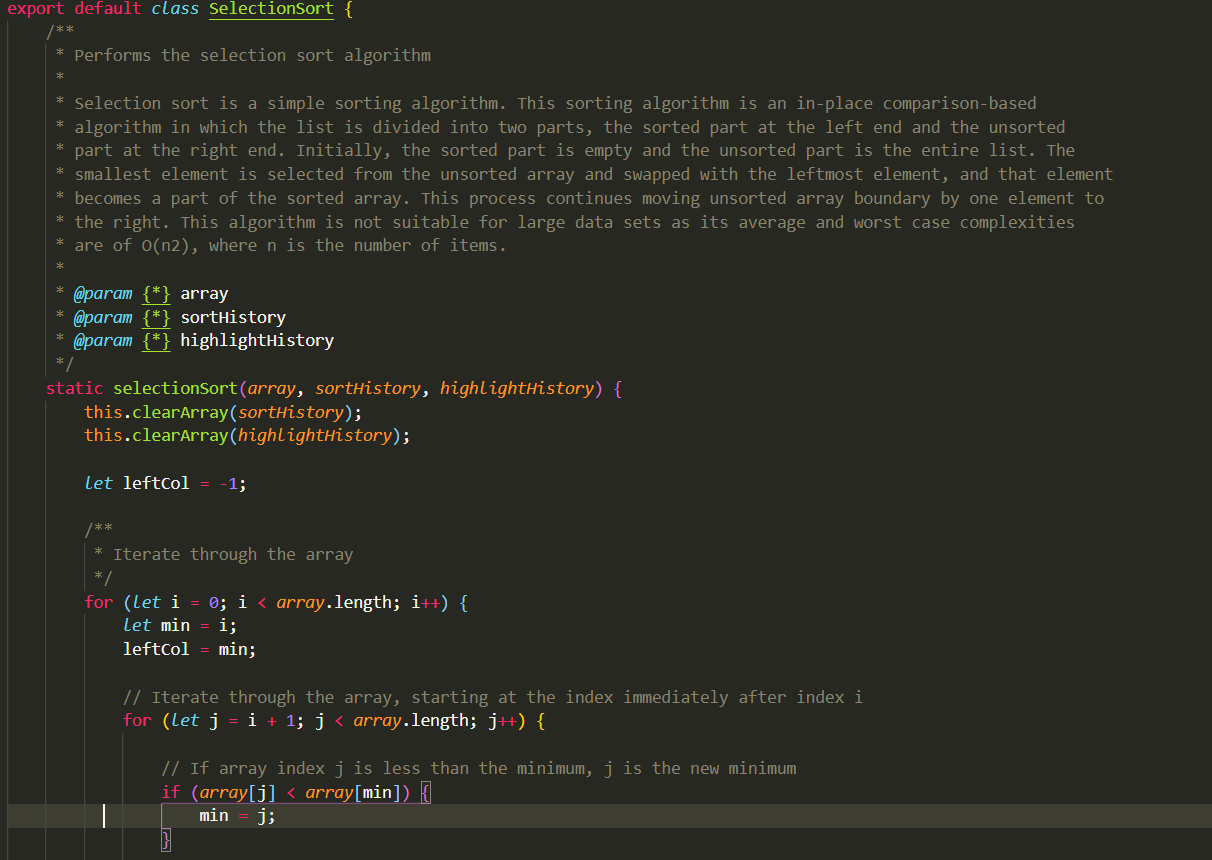
\includegraphics[width=12cm,height=15cm,keepaspectratio]{images/selectionsort1}
    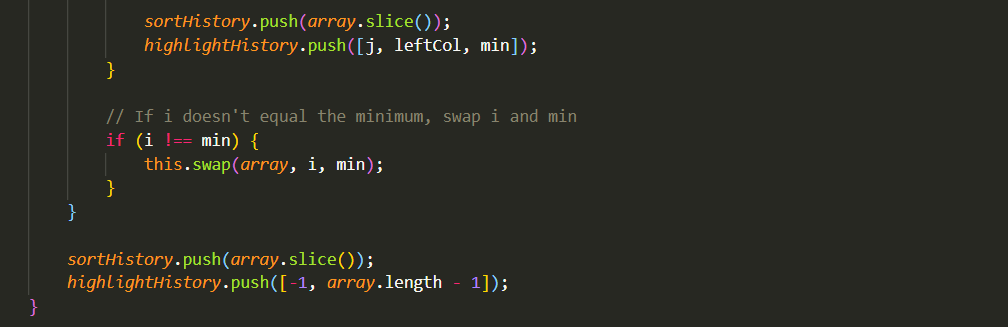
\includegraphics[width=12cm,height=15cm,keepaspectratio]{images/selectionsort2}
\end{center}
Selection sort is an in-place comparison sorting algorithm \cite{selection_sort}. It has an O(n2) time complexity, which makes it inefficient on large lists, and generally performs worse than the similar insertion sort. Selection sort is noted for its simplicity and has performance advantages over more complicated algorithms in certain situations, particularly where auxiliary memory is limited.
\par
\bigskip
The algorithm divides the input list into two parts: a sorted sublist of items which is built up from left to right at the front (left) of the list and a sublist of the remaining unsorted items that occupy the rest of the list. Initially, the sorted sublist is empty and the unsorted sublist is the entire input list. The algorithm proceeds by finding the smallest (or largest, depending on sorting order) element in the unsorted sublist, exchanging (swapping) it with the leftmost unsorted element (putting it in sorted order), and moving the sublist boundaries one element to the right.
\par
\bigskip
The time efficiency of selection sort is quadratic, so there are a number of sorting techniques which have better time complexity than selection sort. One thing which distinguishes selection sort from other sorting algorithms is that it makes the minimum possible number of swaps, n − 1 in the worst case.

\paragraph{How it works in the context of the application}
For the first position in the sorted list, the whole list is scanned sequentially. The whole array is sorted to find the lowest value. After one iteration, the minimum value is stored in the first position of the sorted list. For the second position, the rest of the list is scanned in a linear manner. The same process is applied to the rest of the items in the array \cite{selection_sort_geeks}.

\subsubsection{Shell Sort}
\begin{center}
    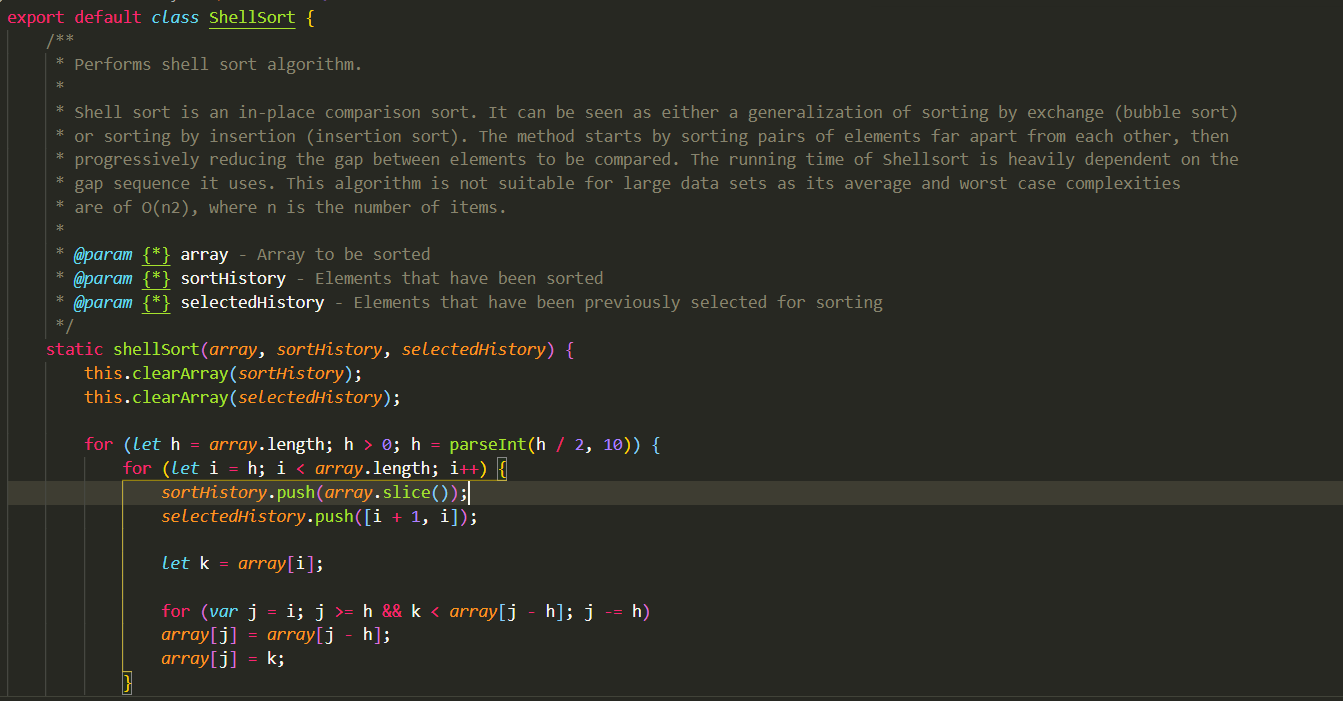
\includegraphics[width=12cm,height=8cm,keepaspectratio]{images/shellsort}
\end{center}
Shell Sort is an in-place comparison sort \cite{shell_sort}. It can be seen as either a generalization of sorting by exchange (bubble sort) or sorting by insertion (insertion sort). The method starts by sorting pairs of elements far apart from each other, then progressively reducing the gap between elements to be compared. Starting with far apart elements, it can move some out-of-place elements into position faster than a simple nearest neighbor exchange. The running time of Shell Sort is heavily dependent on the gap sequence it uses. For many practical variants, determining their time complexity remains an open problem.
\par
\bigskip

\paragraph{How it works in the context of the application}
The idea of Shell Sort is to allow exchange of far items. In Shell Sort, we make the array h-sorted for a large value of h. We keep reducing the value of h until it becomes 1. An array is said to be h-sorted if all sublists of every h’th element is sorted \cite{shell_sort_geeks}.
\par
\bigskip
Bogo Sort and Heap Sort have been programmed as well, however, they are not fully working as of now and as such, they are not covered in this section.

\subsection{Visualization}
\begin{center}
    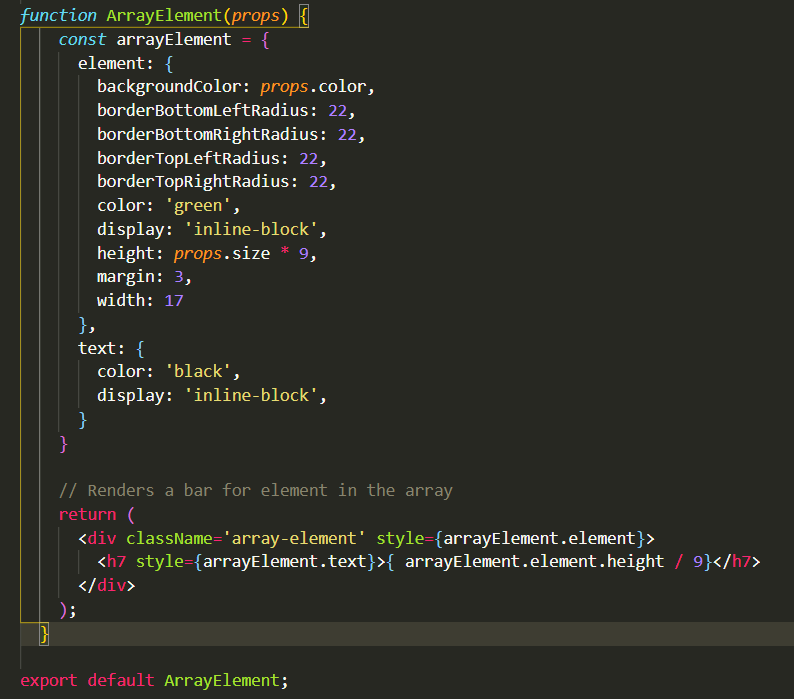
\includegraphics[height=8cm,width=12cm]{images/arrayelement}
    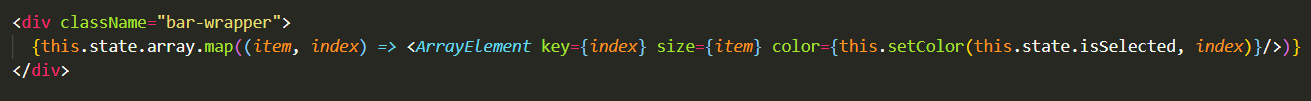
\includegraphics[height=1cm,width=12cm]{images/maparray}
\end{center}
The ArrayElement renders a bar that will represent each element in the array. In MainPage, each element and it's index will be mapped and then visually represented by the bar generated using ArrayElement \cite{react_bar}.

\newpage
\section{Flask Server}
The Flask server, which is hosted on PythonAnywhere, is the middle-man of the entire application and allows the web application to communicate with the database. The server was developed and integrated into the web application secondly alongside the database. It handles requests, such as user login requests, user registration requests, uploading saved sorts, etc. made by the web application and performs the appropriate action. The database is then read and/or updated based on this. 

\begin{center}
    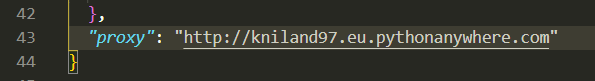
\includegraphics[width=12cm,height=10cm,keepaspectratio]{images/proxy}
\end{center}

\section{Databases}
This application utilizes two databases: a MongoDB database, which is used to store user details and a Firebase database, which stores all previous sorts.

\subsection{MongoDB}
MongoDB was chosen as the database to store user details as MongoDB stores data records as BSON documents. BSON is a binary representation of JSON documents, though it contains more data types than JSON. I thought this would be the best way to save user details since there are several libraries, such as bcrypt, that could work hand-in-hand. The value of a field can be any of the BSON data types, including other documents, arrays, and arrays of documents. 

\begin{center}
    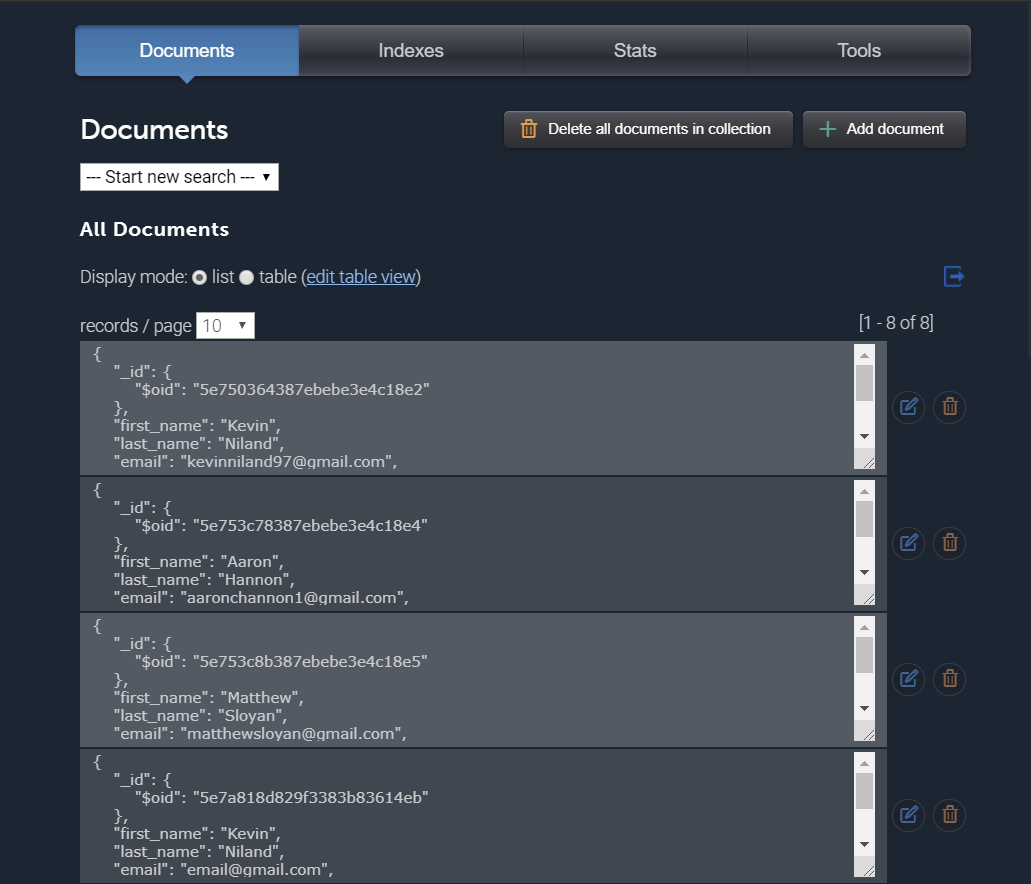
\includegraphics[width=12cm,height=6cm,keepaspectratio]{images/mlab}
\end{center}

\newpage
\subsection{Firebase}
Firebase was chosen as the database to store previous sorts as it provides an easy and simple way to store files. There are a number of React libraries, such as React File Uploader, that have been specifically developed to work with Firebase which provides a simple and easy way to upload a file to Firebase. Firebase itself also provides a number of methods, such as getMetadata() which will retrieve the file type and getDownloadURL() which will retrieve the download URL for each file, that enable an application to retrieve these files easily.

\begin{center}
    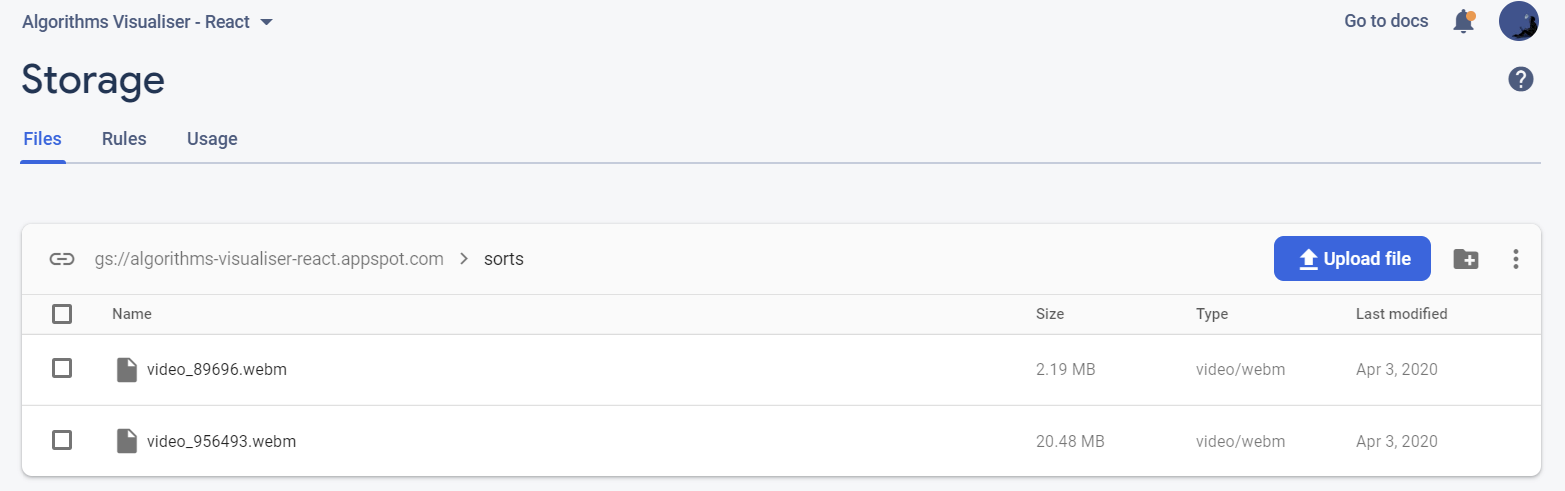
\includegraphics[width=12cm,height=15cm,keepaspectratio]{images/firestore}
\end{center}

Firebase Storage was designed specifically to allow users to upload files, such as images and videos. Data is stored in a Google Cloud Storage bucket, an exabyte scale object storage solution with high availability and global redundancy.